%%%%%%%%%%%%%%%%%%%% ANEXOS / APPENDIX %%%%%%%%%%%%%%%%%%%%%%
\appendix           % appendix starts from here
\appendixpage  		% add a blank page to start the appendix
\addappheadtotoc 	% add appendix to the TOC

\chapter{Reinforcement Learning}
\label{chap:appendix-c1}

\section{Classic learning methods in RL} \label{app:classic_rl}
\subsection{Monte Carlo estimation:} 
Monte Carlo estimation \cite{gerstner2021multilevel} uses complete episodes to approximate the value function using the empirical mean. The value function is based on the returns $G_t$, and since we are trying to approximate $V_{\pi}(s)$, our returns will be the statistic we will use to adjust the value of a state $S_t$. In non-stationary problems, where the environment may change over time, the value function will be incrementally updated as in equation \ref{eq:eq_mc_update}, and by the law of large numbers, if the number of times we visited a state $S$ goes close to infinity, then $V(S) = V_{\pi}(S)$ 

\begin{equation} \label{eq:eq_mc_update}
	V(S_t) \leftarrow V(S_t) + \alpha(G_t - V(S_t))
\end{equation}

Where $\alpha$ is the step-size hyper-parameter that tells the update function how much error take into account in the when performing the adjustments from the estimates. This approach has unbiased but noisy estimations, as the rewards distribution may not be consistent between episodes, creating prone-to-error estimates that may take a long time to converge to the true value function $V_{\pi}(s)$.

\subsection{Temporal Difference Learning:}
TD methods learn from episodic and non-episodic experiences, so the concept of bootstrapping is introduced. Bootstrapping refers to the ability of a model to make an approximation of the value function every each \textit{n-steps}, using the estimation of the returns we have computed as we have collected more and more experience without finishing the current episode. The simplest set-up of TD is TD(0), where we look ahead only one time-step, from $S$ to $S_{t+1}$, and the update for the value function is defined in equation \ref{eq:eq_td0_update}.

\begin{equation} \label{eq:eq_td0_update}
	V(S_t) \leftarrow V(S_t) + \alpha(R_{t+1} + \gamma V(S_{t+1}) - V(S_t))
\end{equation}

Why is this a good idea? imagine a situation where an agent is driving a car, and another car comes towards the agent, but avoids it in the last moment. In the Monte Carlo learning approach, as it learns from complete episodes, the agent would not have learned anything, since the episode ended without much consequences. In TD(0), since it is learning from each time-step, the agent would have learn from the experience itself, and for example, discover that, when a car is approaching, slowing down to have better maneuverability could be an great approach.

Looking just one step in the future might be a little short-sighted, so we can consider to look several steps ahead, considering:

\begin{itemize}
	\item For n = 1 $\rightarrow G^{1}_t = R_{t+1} + \gamma V(S_{t+1})$
	\item For n = 2 $\rightarrow G^{2}_t = R_{t+1} + \gamma R_{t+2} + \gamma V(S_{t+1})$
	\item For n = k $\rightarrow G^{k}_t = R_{t+1} + \gamma R_{t+2} ... \gamma^{k-1}R_{t+k} + \gamma^{k} V(S_{t+k})$
\end{itemize}

What we may not know which n is better, since the search space can be infinite. So the solution that TD($\lambda$) proposes is to have a weighted sum of the returns taking into account different time horizons (equation \ref{eq:lamda_return}), and then use it as our estimation of the value as portrayed in update equation \ref{eq:tdlambda_update}. Figure \ref{fig:td_returns} portrays a visual illustration of how this works.

\begin{equation}\label{eq:lamda_return}
	G^{\lambda}_{t} = (1-\lambda)\sum_{n=1}^{k} \lambda^{n-1}G^{n}_{t}
\end{equation}

\begin{equation} \label{eq:tdlambda_update}
	V(S_t) \leftarrow V(S_t) + \alpha(G^{\lambda}_{t} - V(S_t))
\end{equation}

A few things to comment about the TD($\lambda$) equation is that if $k=\infty$, then we would be in a similar to Monte Carlo learning update, but if $k=1$, then we would end up in the TD(0) update equation.

\begin{figure}[!h]
	\centering
	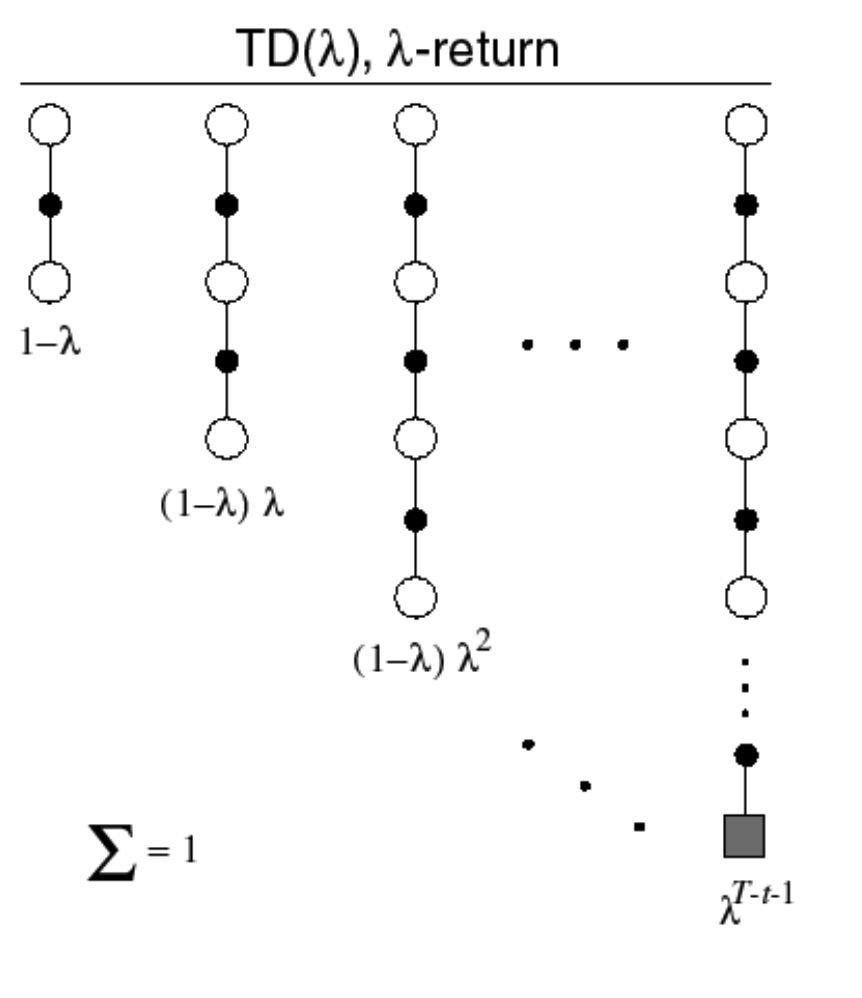
\includegraphics[scale=0.5]{figures/tdlambda_return.png}
	\caption{TD Returns}
	\label{fig:td_returns}
\end{figure}

The policy will use these values to act greedily, as defined in equation \ref{eq:eq_greedy_policy}. Since what it wants to maximize is the value, given the MDP model and the action space $\mathcal{A}$, the policy will select the action that gives more value in future states s'. The issue is that, as stated at the beginning of this section, we are in model-free RL and we no longer have the environment dynamics and $\mathcal{P}$ and reward function $\mathcal{A}$. In the next section we will introduce control, and with it, how the policy problem in tackled.

\begin{equation} \label{eq:eq_greedy_policy}
	\pi'(s) = \operatorname*{argmax}_{a \ni \mathcal{A}} \mathcal{R}^{a}_{s} + \mathcal{P}^{a}_{ss'} V(s')
\end{equation}

\subsection{On-Policy Control: } \label{app:on-policy-control}

On policy RL means that the updates of the value functions are performed according to following a policy $\pi$. Up until this point, everything we have done is evaluate states, and act according to those values. The issue is, that the policy defined in equation \ref{eq:eq_greedy_policy} requires a model of the MDP, and since we are in model-free RL, this is not possible. Instead, we introduce action-value functions, $Q(s,a)$ that take into account, the value of an action, given a state (equation \ref{eq:q_value}).

\begin{equation} \label{eq:q_value}
	q_{\pi}(s,a) = \mathbb{E}_{\pi}[R_{t+1} + \gamma q_{\pi}(S_{t+1},A_{t+1}) | S_t=s , A_t=a]
\end{equation}

Now, we re-write the policy in equation \ref{eq:action_value_policy}, that it still greedy, since we pick the action a that maximizes the action value estimates $Q$, given a state s.

\begin{equation} \label{eq:action_value_policy}
	\pi'(s) = \operatorname*{argmax}_{a \ni \mathcal{A}} {Q}(s,a)
\end{equation}

One thing to note is that, if our policy always acts greedily, then it will never explore other states, since it will always prioritize rewards over landing on new states that may lead to biggest rewards. This is why the $\epsilon$-greedy policy was introduced. This policy acts greedily with a probability of $p = (1 - \epsilon)$ and randomly with a probability $p = \epsilon$. 

Since now we are dealing with action-value functions, we must adapt the TD algorithm. This adaptation is the SARSA algorithm (State-Action-Reward-State-Action) and its update function is shown in equation \ref{eq:sarsa}.

\begin{equation} \label{eq:sarsa}
	{Q}(S,A) \leftarrow {Q}(S,A) + \alpha(R + \gamma{Q}(S',A') - {Q}(S,A))
\end{equation}

\noindent where we define the TD error in equation \ref{eq:td_error}.
\begin{equation} \label{eq:td_error}
	\delta = R + \gamma{Q}(S',A') - {Q}(S,A)
\end{equation}

If we take the approach of TD($\lambda$), we can use SARSA as a along a n-step action-value estimator, instead of just one look-ahead estimator. 

\begin{itemize}
	\item For n = 1 $\rightarrow q^{1}_t = R_{t+1} + \gamma Q(S_{t+1})$
	\item For n = 2 $\rightarrow q^{2}_t = R_{t+1} + \gamma R_{t+2} + \gamma Q(S_{t+1})$
	\item For n = k $\rightarrow q^{k}_t = R_{t+1} + \gamma R_{t+2} ... \gamma^{k-1}R_{t+k} + \gamma^{k} Q(S_{t+k})$
\end{itemize}

And using the same weighted average using the $\lambda$ parameter, we can obtain the SARSA($\lambda$) algorithm, as shown in equation \ref{eq:sarsa_lambda_return}

\begin{equation}\label{eq:sarsa_lambda_return}
	q^{\lambda}_{t} = (1-\lambda)\sum_{n=1}^{k} \lambda^{n-1}q^{n}_{t}
\end{equation}

\begin{equation} \label{eq:sarsa_lambda}
	{Q}(S_t,A_t) \leftarrow {Q}(S_t,A_t) + \alpha(q^{\lambda}_{t} - {Q}(S_t,A_t))
\end{equation}

\subsection{Off-Policy Control: } \label{app:on_policy_control}

Dealing with just one policy, $\pi$, may limit the scope of learning. To put a easy example, it would be as if humans would only learn following a single philosophy. It is not a bad approach, but as we add new perspectives to our learning process, better outcomes come out of it (i.e. work, university, relationships). Off-policy learning, among other motives, was introduce to make the agent more flexible in the learning process, taking into account different perspectives and explore while learning the optimal policy. In off-policy learning, usually there are two policies: the target policy $\pi$ that is used to compute the ${Q}$ values, and the behavioural policy $\mu$, which usually has an exploratory component to it.

One of the most famous algorithms that implements off-policy learning is Q-learning \cite{Watkins1992}. It is mainly divided in three blocks:

\begin{enumerate}
	\item The next action $A_{t+1}$ is selected following the behaviour policy $\mu(A|S_t)$
	\item The alternate action A' is selected following the target policy $\pi(A|S_t)$
	\item Use the update equation (eq. \ref{eq:q_leaning}) to update the action-values ${Q}$.
\end{enumerate}

\begin{equation} \label{eq:q_leaning}
	{Q}(S_t, A_t) \leftarrow {Q}(S_t, A_t) + \alpha[R_{t+1} +  \operatorname*{max}_{a'}\gamma{Q}(S_{t+1}, a') - {Q}(S_t, A_t)]
\end{equation}

\subsection{Actor-Critic Methods}
\label{sec:ac-methods}
Currently, the most common policy gradient methods are based on actor-critic methods. The critic (action-value function) makes evaluations of the actor's actions using function approximation $\hat{{Q}}_{w}(s,a)$. The actor tries actions and optimize them in the direction the critic proposes. This is formalized in equation \ref{eq:actor-critic} where the approximation of the policy gradient takes into account the action-value function as part of the update.

\begin{equation}\label{eq:actor-critic}
	\Delta\theta_{t} = \alpha(\nabla_{\theta} log \pi_{\theta}(s,a)\hat{{Q}}_{w}(s,a))
\end{equation}

One thing to note is that in this method we have two approximators, hence, two set of parameters, w and $\theta$. The most recent actor critic methods follow this principle, but add different optimization tools to obtain more stable and robust results in the policy learning process.

\begin{itemize}
	\item Soft Actor-Critic (SAC) \cite{haarnoja2018soft}: SAC is another off-policy actor-critic algorithm that incorporates maximum entropy reinforcement learning. It maximizes the expected return while also maximizing entropy, leading to policies that are more exploratory and robust. Right now is the state-of-the-art method for policy optimization.
	\item Proximal Policy Optimization (PPO) \cite{schulman2017proximal}: PPO is an actor-critic method that addresses the limitations of previous policy gradient methods. This is done by limiting the policy update to be close to the previous policy, helping to stabilize training and preventing large policy updates which may lead to performance degradation.
	\item Deep Deterministic Policy Gradient (DDPG) \cite{lillicrap2019continuous}: DDPG is an off-policy actor-critic algorithm specifically designed for continuous action spaces. This are spaces where the set of actions may be infinte, and a greedy (max) policy do not work. It learns a deterministic policy function using deep neural networks to approximate the Q-function and the policy.
\end{itemize}

\chapter{Attention Mechanism}

\section{Understanding the attention mechanism}
\label{app:attention-mec}

The attention mechanism appeared as a learnable alignment method for the translation task. This sequence to sequence problem had a weakness in the recursive neural network set-up. Up until that point, the way this kind of problem was addressed was by using a bidirectional RNN (usually a bi-LSTM) in the encoder, that tried to compress the information from the whole sequence in the hidden state vector from the LSTM. This was done forward and backwards to then concatenate the hidden state vectors from both LSTMs into one joint vector. This is defined in equation \ref{eq:bi_hidden_vector}

\begin{equation}
	\label{eq:bi_hidden_vector}
	\textbf{h}_1, ..., \textbf{h}_t = \text{bi-RNN}(x_1, ..., x_t)
\end{equation}

where $\textbf{h}_i$ is computed like shown in equation \ref{eq:h_vector}, where the notation $\{\cdot ; \cdot\}$ represents the concatenation between two vectors.

\begin{equation}
\begin{split}
	\label{eq:h_vector}
	\overrightarrow{h_i} = RNN_{forward}(x_i) \\
	\overleftarrow{h_i}  = RNN_{backward}(x_i) \\
	\textbf{h}_i = \{\overrightarrow{h_i};\overleftarrow{h_i}\}
\end{split}
\end{equation}

After that, the encoder, usually another RNN, would use the joint vector  $\textbf{h}_i$ to "decode" the sequence into the desired output (i.e.  the translated version of the input). As one could sense, compressing the information of big sequences becomes a problem when the hidden vector is of fixed size. What the attention mechanism proposed, was a way to dynamically change the hidden vector as the sequence was processed and new context from the input was acquired.

Bahdanu \textit{et al.} used the same set-up in the encoder in \cite{bahdanau2016neural}, but introduced new modifications at the decoder to make the hidden vector change over the time-steps of the sequence. To do so, they introduced the attention block, where the context vector $\textbf{c}_t$ is computed for each time step \textit{t}. This vector represents the relationship between the current output symbol and each term that belongs to the input sequence. Details on how the context vector $\textbf{c}_t$ is computed are at equation \ref{eq:context_vector_comp}

\begin{equation}
	\label{eq:context_vector_comp}
	c_t = \sum_{j=1}^{T} \alpha_{tj} \cdot \textbf{h}_j
\end{equation}

Where $\alpha_{tj}$ is a scalar that represents the weight of the hidden state vector $ \textbf{h}_j$ over the final context vector in time-step t. As one can interpret from equation \ref{eq:context_vector_comp},  $\alpha_{t}$ contains the information for all the input tokens processed up to the j-th element, hence, it will change its values for each time-step. Also, to prevent the decoder to "look ahead" of the sequence, the inputs tokens that are after the  j-th element in the sequence will be masked, so that the attention block cannot take them into account. The computation of  $\alpha_{tj}$ is showed in equation \ref{eq:weigth_comp}, where $s_{t-1}$ is the hidden state of the decoder at time-step t-1 and $f$ is a learnable function (i.e. a neural network) that outputs the logit (or energy, as they call it in the original work) $e_{tj}$, that ponders how much correlation exists between vectors $h_j$ and $s_{t-1}$. This correlation is then normalized by using the softmax function, producing the value $\alpha_{tj}$.

\begin{equation}
	\label{eq:weigth_comp}
	\begin{split}
		\alpha_{tj} = \frac{\text{exp}(e_{tj})}{\sum_{k=1}^{T} \text{exp}(e_{tk})} \\
		e_{tj} = f(s_{t-1}, h_j)
	\end{split}
\end{equation}

Finally, after all the alignments are computed, the RNN from the decoder outputs the most probable symbol $y_t$ at the current time-step $t$ (equation \ref{eq:dec_out_probs}).

\begin{equation}
	\label{eq:dec_out_probs}
	\mathbb{P}(y_t | y_{t-1}, ..., y_1, x) = RNN_{decoder} (c_t)
\end{equation}

\section{From attention to self-attention}
\label{from_att_2_selfatt}
Results from the attention encoder decoder architecture were a leap of performance with respect to previous work, but they still failed to perform correctly as the number of tokens in the input sequence increased. To tackle this problem, Vaswani \textit{et al.} proposed a different approach. Instead of the neural network processing one token at each time-step and compressing the information in a single hidden state vector iteratively, the sequence is processed as a whole, and each of the input tokens compute how relevant the other tokens are with respect to themselves. This mechanism is called self-attention.

To implement this mechanism, the authors propose to operate with three terms, the query Q, the keys K and the values V. These values are computed by projecting the original embeddings from the input $X \in \mathbb{R}^{n \times d}$, where n is the number of tokens in the input sequence and d is the embedding dimension, to the three matrices such that $Q = XW^Q$, $K = XW^K$ and $V = XW^V$. For clarification, $W^Q, W^K$ and $W^V \in  \mathbb{R}^{d \times d_k}$, where $d_k$ represents the dimension of the new space where $X$ is projected to compute $Q, K$ and $V$.

To follow the same terminology used in section \ref{app:attention-mec}, we are going to dissect the compact form of the attention defined in equation \ref{eq:app_self_attn} into the several parts so that resembles the way that the "classic" attention mechanism is computed.

\begin{equation}
	\label{eq:app_self_attn}
	\text{Attention}(Q, K, V) = \text{softmax}\left(\frac{QK^\top}{\sqrt{d_k}}\right) V
\end{equation}

In section \ref{app:attention-mec} we explained how the context vector $c_j$ contained the compressed information of the pondered sum from all the input tokens up to the j-th element of the sequence. On a similar fashion, the self-attention mechanism computes the context vector by projecting the j-th token of the input sequence, $x_j$, into a new space using $W^V$ and then pondering it with respect to the rest of the i-th elements from the sequence by multiplying them times $\alpha_{ij}$. As in the "classic" attention, $\alpha_{ij}$ is the normalized correlation between the i-th element and the j-th, and it is done by applying the softmax function, as shown in equation \ref{eq:self_attn_weigth_comp}, but the way $e_{i\cdot}$ is computing differs.

\begin{equation}
	\label{eq:self_attn_weigth_comp}
	\begin{split}
		\alpha_{ij} = \frac{\text{exp}(e_{ij})}{\sum_{k=1}^{n} \text{exp}(e_{ik})}
	\end{split}
\end{equation}

To compute the $e_{i\cdot}$ the self-attention formula proposes the scaled-dot product as the compatibility function. This function aims to give a magnitude of how correlated are two vectors from the input, since the dot product is greater the closer two vectors are on an euclidean space. Following this principle, we assume that the tokens that are similar semantically, will be closer in the embedding space, thus producing a greater value. The "scaled" part (i.e. $\frac{1}{\sqrt{d_z}}$)tries to stabilize the softmax function in terms of saturation, by preventing the values of the vectors from getting too big. This function is showed in equation \ref{eq:com_function_self_attn}, where $\cdot$ represents the dot-product between the i-th element in the query space and the j-th element in the key space, projected by the matrix-vector multiplication of their respective query and key projection matrices.

\begin{equation}
	\label{eq:com_function_self_attn}
	e_{ij} = \frac{(x_i W^Q)\cdot(x_j W^K)}{\sqrt{d_z}}
\end{equation}

Finally, to compute the attention-pondered final values $z_i$, we will multiply the weight values $\alpha_{ij}$ by each of the elements of the input $X$ after they are projected into the value space. Finally, we add them up, hence obtaining equation \ref{eq:final_attn_weights}.

\begin{equation}
	\label{eq:final_attn_weights}
	e_{ij} = \sum_{j=1}^{n} \alpha_{ij}(x_j) W^V
\end{equation}

As a final reflection, if we pay a closer look to equations \ref{eq:weigth_comp} and \ref{eq:com_function_self_attn}, we see that the mechanism is practically the same, where $h_i$ are the keys, and $s_{t-1}$ are the queries and the operations between them are practically the same, since $h_i$ and $s_{t-1}$ are the encoded information from the sequence in the embedded space. Something similar occurs with equations \ref{eq:final_attn_weights} and \ref{eq:context_vector_comp} where the value matrix is equivalent the $h_j$ vector at the input of the decoder. Here we can see that the relationship between the attention decoder and the self-attention mechanism from the transformer model lie under the same principles, compute which parts of the input are more relevant in terms of context to produce the appropriate output.

\chapter{Schedulers}
\label{app:gamma_proof}

\section{Gamma for the exponential equation}
As explained in section \ref{sec:digging_dqn_agent}, the equation we must solve for gamma is the following: 
\begin{equation}
	\epsilon_t = \epsilon_0 \gamma^{\lambda t}
\end{equation}

But, since we want the equation to be bounded between $\epsilon_0$ and $\epsilon_f$ in the domain $[0, N]$, so we must substitute $\epsilon_t$ by $\epsilon_f$. Additionally, since we want the value of $\epsilon_t = \epsilon_f$ when $t = N$, then we substitute it accordingly in the equation.

\begin{align}
	\epsilon_f &=  \epsilon_0 \gamma^{\lambda N} \quad \text{(Original equation)} \label{eq1} \\
	\frac{\epsilon_f}{\epsilon_0} &= \gamma^{\lambda N} \quad \text{(Divide by $\epsilon_0$ in both sides)} \label{eq2} \\
	\sqrt[\lambda N]{\frac{\epsilon_f}{\epsilon_0}} &= \gamma \quad \text{(Exponentiation in both sides by $\frac{1}{\lambda N}$ )} \label{eq3} 
\end{align}

Hence, obtaining $\gamma$ for the exponent function.

\section{Gamma for the product of exponential equation}
Introducing again the equation in \ref{sec:digging_dqn_agent}, now we must solve for gamma: 
\begin{equation}
	\epsilon_f = \epsilon_0 \prod_{i=0}^{N} \gamma^{\lambda i}
\end{equation}

\noindent Lets begin with the procedure:
\begin{align}
	\epsilon_f &= \epsilon_0 \prod_{i=0}^{N} \gamma^{\lambda i} \quad \text{(Original equation)} \label{eq4} \\
	\frac{\epsilon_f}{\epsilon_0} &= \prod_{i=0}^{N} \gamma^{\lambda i} \quad \text{(Divide by $\epsilon_0$ in both sides)} \label{eq6} \\
	\log_\gamma \left(\frac{\epsilon_f}{\epsilon_0}\right) &= \log_\gamma \left( \prod_{i=0}^{N} \gamma^{\lambda i} \right) \quad \text{(Apply logarithms to both sides)} \label{eq7} \\
	\log_\gamma \left(\frac{\epsilon_f}{\epsilon_0}\right) &= \sum_{i=0}^{N} \log_\gamma  \gamma^{\lambda i} \quad \text{(By the product property of logarithms)} \label{eq9} \\
	\log_\gamma \left(\frac{\epsilon_f}{\epsilon_0}\right) &= \sum_{i=0}^{N} \lambda i \log_\gamma \gamma \quad \text{(By the exp. property of logarithms)} \label{eq10} \\
	\log_\gamma \left(\frac{\epsilon_f}{\epsilon_0}\right) &= \sum_{i=0}^{N} \lambda i \quad \text{(Simplifying logarithms)} \label{eq11} \\
	\log_\gamma \left(\frac{\epsilon_f}{\epsilon_0}\right) &= \lambda \sum_{i=0}^{N} i \quad \text{(Taking the constant out of the sum)} \label{eq12} 
\end{align}

Let $\sum_{i=0}^{N} i = k$, then we can compute it using the general summation formula:
\begin{equation}
	\label{eq:gen_sum}
	k = \sum_{i=0}^{N} i  = n a_1 + d \frac{(n-1)n}{2}
\end{equation}

Where $n$ is the final value, $a_1$ is the first value and $d$ is the interval between the numbers of the sum. Then, by substituting \ref{eq:gen_sum} in \ref{eq12}, we get the following:
\begin{align}
	\log_\gamma \left(\frac{\epsilon_f}{\epsilon_0}\right) &= \lambda k \quad \label{eq13}
\end{align}

And by the definition of a logarithm $\log_b(x) = y \Leftrightarrow b^y = x$, we can express equation \ref{eq13} as:

\begin{align}
	\left(\frac{\epsilon_f}{\epsilon_0}\right) &= \gamma^{\lambda k} \quad \text{(Applying the definition of a logarithm)} \label{eq14} \\
	\sqrt[\lambda k]{\frac{\epsilon_f}{\epsilon_0}} &=\gamma \quad \text{(Exponentiation of both sides by $\frac{1}{\lambda k}$)} \label{eq15}
\end{align}

Hence, obtaining $\gamma$ for the product of exponents function.
